\section{ Хеш-функции. Коллизии. Хеш-таблицы.  Хеширование. Фильтр Блюма.}

\subsection*{Хеш-таблица}
\textbf{Хеш-таблица} --- это эффективная структура данных для реализации ассоциативных массивов. Используется, когда количество реально хранящихся в массиве ключей мало по сравнению с количеством значений ключей. Она использует массив, размер которого кратен количеству реально хранящихся в нём ключей.

\textbf{Ассоциативный массив} --- это абстрактный тип данных, состоящий из пар "ключ-значение". Ключ уникален, для него введена операция сравнения.

\begin{figure}[h!]
	\centering
	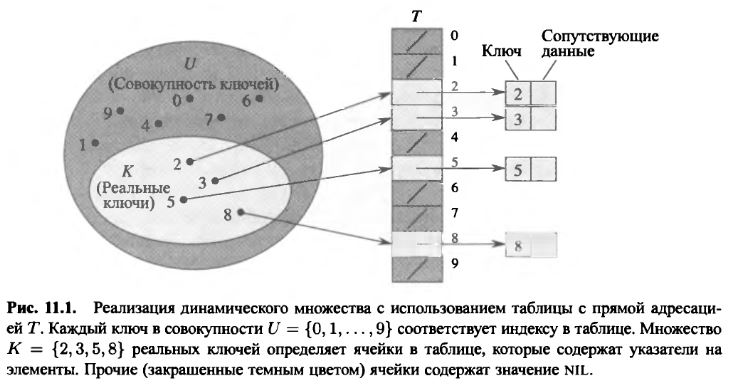
\includegraphics[width=0.4\linewidth]{img_easy/11_2.png}
	\captionsetup{labelformat=empty}
	\caption{Ассоциативный массив}
\end{figure}

Вместо использования ключа в качестве индекса, хэш-таблица вычисляет индекс по значению ключа. Это позволяет избежать потери памяти.

\subsection*{Коллизии}
Таблица с прямой адресацией: элемент ключа $k$ хешируется в ячейку $h(k)$. Величина $h(k)$ называется хеш-значением ключа $k$.

\textbf{Принцип Дирихле (в контексте хеш-таблиц)} означает ситуацию, называемую коллизией: когда по двум ключам доступна одна и та же ячейка.

\subsubsection*{Способы разрешения коллизий:}
\begin{enumerate}
	\item \textbf{Хеш-таблицы с цепочками}:
	Каждая ячейка $h(k)$ хранит список (цепочку) элементов, которые хешируются в эту ячейку.
	\begin{itemize}
		\item Операции:
		\begin{enumerate}
			\item Вставка: $O(1)$. Вычисляем $h(k)$, вставляем элемент в начало списка, связанного с ячейкой $h(k)$.
			\item Поиск: Вычисляем $h(k)$, поиск в соответствующем списке.
			\item Удаление: $O(t)$. Поиск ключа $k$, удаление в случае успеха.
		\end{enumerate}
		\item Сложность: Если количество элементов в цепочке в среднем одинаково $C_k = n/m$ (где $n$ - количество ключей, $m$ - длина хеш-таблицы), то сложность операций $O(1)$.
	\end{itemize}
	
	\item \textbf{Хеш-таблицы с открытой адресацией}:
	Все элементы хранятся непосредственно в хеш-таблице, без использования связанных списков.
	\begin{itemize}
		\item Для разрешения коллизий: ищем пустую ячейку и добавляем туда.
		\item Если таблица полностью заполнена, увеличиваем её размер.
		\item \textbf{Стратегии поиска пустой ячейки}:
		\begin{enumerate}
			\item Линейный поиск: просматриваем ячейки $i, i+1, i+2, \dots$ пока не найдём свободную.
			\item Квадратичный поиск: смещение не фиксировано, а изменяется квадратично (например, $1, 4, 9, 16, \dots$). Просматриваем $i+1, i+4, i+9, \dots$.
		\end{enumerate}
	\end{itemize}
	
	\subsection*{Хеш-функции}
	\subsubsection*{Метод деления}
	$h(k) = k \pmod m$. Выбираем $m$ простым, далёким от степени 2.
	
	\textbf{Пример:} $m=13$
	\begin{itemize}
		\item $K_1 = 1 \rightarrow h(K_1) = 1$
		\item $K_2 = 100 \rightarrow h(K_2) = 9$
		\item $K_3 = 12 \rightarrow h(K_3) = 12$
		\item $K_4 = 179 \rightarrow h(K_4) = 10$
		\item $K_5 = 2 \rightarrow h(K_5) = 2$
		\item $K_6 = 444 \rightarrow h(K_6) = 2$ 
	\end{itemize}
	
	\subsubsection*{Метод умножения}
	$h(K) = \lfloor m (K \cdot A \pmod 1) \rfloor$.
	Желательно, чтобы $A$ не была дробной частью часто числа. $A \in \mathbb{R}$, $0 < A < 1$.
\end{enumerate}

\begin{definition}
	\textbf{Фильтр Блума} --- вероятностная структура данных позволяющая проверять принадлежность элемента к множеству. 
	При этом существует возможность получить \textbf{ложноположительное} срабатывание (элемента в множестве нет, но структура данных сообщает, что он есть), но не \textbf{ложноотрицательное}.
\end{definition}

То есть данный фильтр даёт два ответа на вопрос о принадлежности элемента к множеству:
\begin{enumerate}
	\item элемент точно не принадлежит множеству,
	\item элемент возможно принадлежит множеству.
\end{enumerate}

Фильтр Блума представляет собой битовый массив из $m$
бит и $k$ различных хеш-функций $h_1 ... h_k$, равновероятно отображающих элементы исходного множества во множество $\{0,1, m-1\}$, соответствующее номерам битов в массиве. 
Изначально, когда структура данных хранит пустое множество, все $m$ бит обнулены.

\begin{figure}[h!]
	\centering
	\includegraphics[width=0.4\linewidth]{img_easy/11_1.png}
	\captionsetup{labelformat=empty}
	\caption{Пример фильтра Блума}
\end{figure}

Для добавления элемента $e$ необходимо записать единицы на каждую из позиций $h_1(e)...h_k(e)$ битового массива.

При поиске элемента необходимо проверить наличие единиц на позициях $h_1(e)...h_k(e)$ --- если хотя бы на одной позиции не будет единицы, элемент точно не присутствует в множестве; п